\documentclass[article]{jlreq}
\usepackage{mathtools, amssymb}
\usepackage{tikz}
\usetikzlibrary{automata,positioning,arrows.meta}

\title{オートマトン・言語理論 レポート課題01}
\author{C5TB2006 安倍大陽}
\date{\today}



\begin{document}


\maketitle


\subsection{\( L_1 = \{w \in \Sigma ^ * \mid \langle w\rangle_a = 2k, k \in \mathbb{N} \}\)}
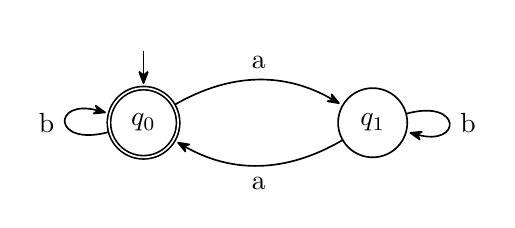
\begin{tikzpicture}[
	->,
	>={Stealth[round]},
	initial text=,
	auto,
	node distance=2cm,
	shorten >=1px,
	semithick,
	inner sep=4px
	]
	\node[state, initial, initial above, accepting] (q_0) {$q_0$};
	\node[state] (q_1) [right=of q_0] {$q_1$};
	\path[->]
	(q_0) edge [bend left] node {a} (q_1)
	edge [loop left] node {b} ()
	(q_1) edge [bend left] node {a} (q_0)
	edge [loop right] node {b} ();
\end{tikzpicture}



\subsection{\( L_2 = \{w \in \Sigma ^ * \mid \langle w\rangle_b = 2k+1, k \in \mathbb{N} \}\)}
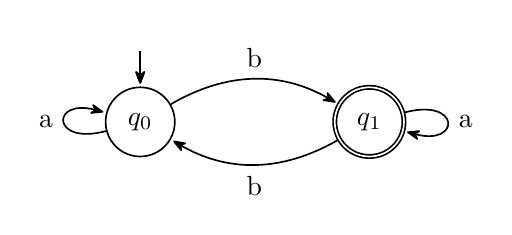
\begin{tikzpicture}[
	->,
	>={Stealth[round]},
	initial text=,
	auto,
	node distance=2cm,
	shorten >=1px,
	semithick,
	inner sep=4px
	]
	\node[state, initial, initial above] (q_0) {$q_0$};
	\node[state, accepting] (q_1) [right=of q_0] {$q_1$};
	\path[->]
	(q_0) edge [bend left] node {b} (q_1)
	edge [loop left] node {a} ()
	(q_1) edge [bend left] node {b} (q_0)
	edge [loop right] node {a} ();
\end{tikzpicture}



\subsection{\( L_3 = \{ w \in \Sigma ^ * \mid \langle w\rangle_a = 3k, k \in \mathbb{N} \}\)}
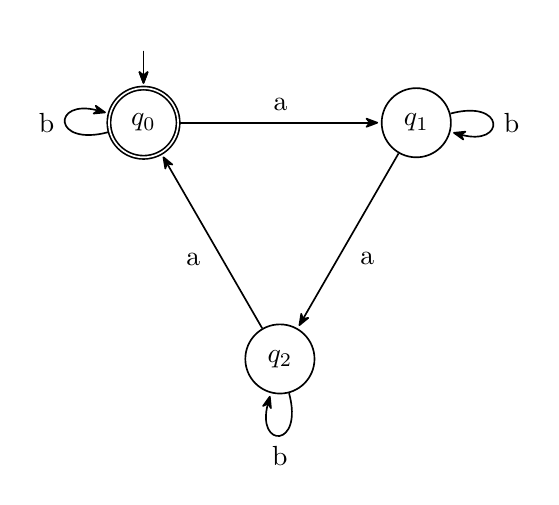
\begin{tikzpicture}[
	->,
	>={Stealth[round]},
	initial text=,
	auto,
	shorten >=1px,
	semithick,
	inner sep=4px
	]
	\node[state, initial, initial above, accepting] (q_0) at (150:2cm) {$q_0$};
	\node[state] (q_1) at (30:2cm) {$q_1$};
	\node[state] (q_2) at (270:2cm) {$q_2$};
	\path[->]
	(q_0) edge node {a} (q_1)
	edge [loop left] node {b} ()
	(q_1) edge node {a} (q_2)
	edge [loop right] node {b} ()
	(q_2) edge node {a} (q_0)
	edge [loop below] node {b} ();
\end{tikzpicture}



\subsection{\( L_4 = \{ w \in \Sigma ^ * \mid \langle w\rangle_b = 3k+2, k \in \mathbb{N} \}\)}
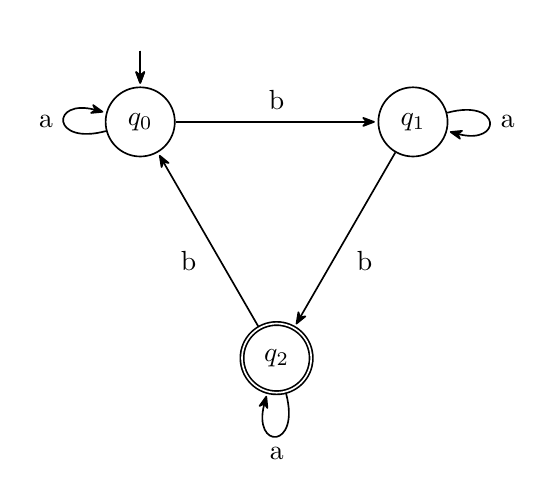
\begin{tikzpicture}[
	->,
	>={Stealth[round]},
	initial text=,
	auto,
	shorten >=1px,
	semithick,
	inner sep=4px
	]
	\node[state, initial, initial above] (q_0) at (150:2cm) {$q_0$};
	\node[state] (q_1) at (30:2cm) {$q_1$};
	\node[state, accepting] (q_2) at (270:2cm) {$q_2$};
	\path[->]
	(q_0) edge node {b} (q_1)
	edge [loop left] node {a} ()
	(q_1) edge node {b} (q_2)
	edge [loop right] node {a} ()
	(q_2) edge node {b} (q_0)
	edge [loop below] node {a} ();
\end{tikzpicture}

\end{document}
